\documentclass[whitelogo]{TUD-report2020}

\usepackage[style=apa]{biblatex}
\addbibresource{report.bib}
\usepackage{hyperref}
\usepackage{changes}


\begin{document}

%% Use Roman numerals for the page numbers of the title pages and table of
%% contents.
\frontmatter

%% Uncomment following 19 lines for a cover with a picture on the lower half only
%\title[tudelft-white]{Title}
%\subtitle[tudelft-cyan]{Optional subtitle}
%\author[tudelft-white]{J.\ Random Author}
%\affiliation{Technische Universiteit Delft}
%\coverimage{cover.jpg}
%\titleoffsetx{10cm}
%\titleoffsety{10cm}
%\afiloffsetx{1cm}
%\afiloffsety{18cm}
%\covertext[tudelft-white]{
%    \textbf{Cover Text} \\
%    possibly \\
%    spanning 
%    multiple 
%    lines
%    \vfill
%    ISBN 000-00-0000-000-0
%}
%\makecover

%% Uncomment following 16 lines for a cover with a picture on the lower half only
\title[tudelft-white]{MSc Graduation Guide}
\subtitle[tudelft-black]{at KAS Lab}
\author[tudelft-white]{Knowledge-based Autonomous Systems Laboratory}
\affiliation{Technische Universiteit Delft}
% \coverimage{tank.jpg}
\coverimage{figures/DALL_E_20221222_robotreadingaboutknowledgerepresentationandsymbolicreasoning.jpg}
\covertext[tudelft-white]{
    \textbf{Authors:} \\
    Carlos Hernandez Corbato
    \vfill
    \today
}
\setpagecolor{tudelft-cyan}

\makecover[split]


%% Include an optional title page.
\begin{titlepage}


\begin{center}

%% Insert the TU Delft logo at the bottom of the page.

%% Print the title in cyan.
{\makeatletter
\largetitlestyle\fontsize{64}{94}\selectfont\@title
%\largetitlestyle\color{tudelft-cyan}\Huge\@title
\makeatother}

%% Print the optional subtitle in black.
{\makeatletter
\ifx\@subtitle\undefined\else
    \bigskip
   {\tudsffamily\fontsize{22}{32}\selectfont\@subtitle}    
    %\titlefont\titleshape\LARGE\@subtitle
\fi
\makeatother}

\bigskip
\bigskip

by
%door

\bigskip
\bigskip

%% Print the name of the author.
{\makeatletter
%\largetitlefont\Large\bfseries\@author
\largetitlestyle\fontsize{26}{26}\selectfont\@author
\makeatother}

\bigskip
\bigskip

% to obtain the degree of Master of Science
% %ter verkrijging van de graad van Master of Science

% at the Delft University of Technology,
% %aan de Technische Universiteit Delft,

% to be defended publicly on Tuesday January 1, 2013 at 10:00 AM.
%in het openbaar de verdedigen op dinsdag 1 januari om 10:00 uur.

\vfill

% \begin{tabular}{lll}
%     Student number: & 1234567 \\
%     Project duration: & \multicolumn{2}{l}{March 1, 2012 -- January 1, 2013} \\
%     Thesis committee: & Prof.\ dr.\ ir.\ J.\ Doe, & TU Delft, supervisor \\
%         & Dr.\ E.\ L.\ Brown, & TU Delft \\
%         & Ir.\ A.\ Aaronson, & Acme Corporation
% \end{tabular}
%% Only include the following lines if confidentiality is applicable.

\bigskip
\bigskip
\emph{license text}
%\emph{Op dit verslag is geheimhouding van toepassing tot en met 31 december 2013.}

\bigskip
\bigskip
An electronic version of this document is available at \url{http://}.
%\\[1cm]

%\centering{
\includegraphics{cover/logo_black}}


\end{center}

\begin{tikzpicture}[remember picture, overlay]
    \node at (current page.south)[anchor=south,inner sep=0pt]{
        
\includegraphics{cover/logo_black}
    };
\end{tikzpicture}

\end{titlepage}



% \chapter*{Preface}
\setheader{Preface}

Preface\ldots

\begin{flushright}
{\makeatletter\itshape
    \@author \\
    Delft, January 2013
\makeatother}
\end{flushright}



\tableofcontents

%% Use Arabic numerals for the page numbers of the chapters.
\mainmatter

\chapter{Introduction}

\section{Who is this guide for?}

This document has been written for master students intending to graduate at the KAS Laboratory, section Robot Dynamics of the department Cognitive Robotics (Faculty 3mE, TU Delft). Typically, these include MSc students from the MSc Robotics \url{https://www.tudelft.nl/onderwijs/opleidingen/masters/robotics/msc-robotics/programme} or BioMechanical Engineering (specialisations BioRobotics). Exceptionally, we supervise students from other backgrounds as well. 
Nonetheless, the guide contains a lot of general tips and tricks that can be applied in other domains.

Disclaimer: this guide is heavily based on the "Master Thesis Guide
Written by Delft Haptics Lab members" (version June 9 2020). We are very grateful to them for sharing such a beautiful guide, and hope there are ok with us reusing parts of it for the KAS Lab guide.

\section{Why this guide?}

A graduation project is a \textit{process}, and as a student typically you have not done it before.
This process covers most of your second year of your MSc, from finding a thesis supervisor and a topic, to eventuelly presenting and defending your project.

This guide is intended to help you in that process. 

% FROM HRI Manual
% Note that an MSc thesis project is not a straightforward affair to which a step-by-step ‘manual’ can be applied. As such, this guide is no more than a guide, it provides a structured approach, examples, and helpful tips \& tricks, but that does not mean this is the only way to go about your thesis project. Please also make use of other guides, tips, tricks, conversations with students & staff, and of course your own creativity and common sense.

\section{Overview of the graduation process and this guide}

\begin{list}
    % \item Chapter \ref{}
    % \item Chapter \ref{}
    % \item Chapter \ref{}
    % \item Chapter \ref{}
\end{list}

\chapter{Workflow and Tools}\label{c:workflow-tools}

\textit{This section is inspired by the \href{https://biaslab.github.io/research/starter-guide/}{Starter's Guide for students at BIASlab research team} by Prof de Vries at the BIASlab group of TU Eindhoven.}

We work together asynchronously, using tools like MS Teams (for communication and data management) and github (for source code version control)

\section{MS Teams}

\subsection{Reporting: LaTeX and Overleaf}
The project’s final report should be written in LaTeX on Overleaf. You must get familiar with LaTeX early during your project, because we start writing the final report very soon after the start of the project.

\subsection{Reference management: Zotero}
After you join the KAS Lab team you will also get access to our literature collection that we store online in a Zotero repository. This will help you get an overview of all relevant papers in our field.



\chapter{Literature Review}\label{c:literature}

\section{What is a Literature Review}
Literature Research is also referred to as Literature Study or Literature Review.
It is individual work on a topic agreed upon between the thesis supervisor and the student.
It involves creating a research question that can be answered using the existing literature, finding and analyzing the right literature, and writing a solid report about it.

% FROM HRI MANUAL
This chapter aims to give guidelines and suggestions to help you in writing your literature report. Typically the report writing takes three months and can roughly be divided into three phases, each requiring approximately one month’s work:
\begin{enumerate}
    \item Orientation \& exploration.
    \item Structured literature search.
    \item Literature documentation.
\end{enumerate}

\begin{figure}[h!]
	\centering
	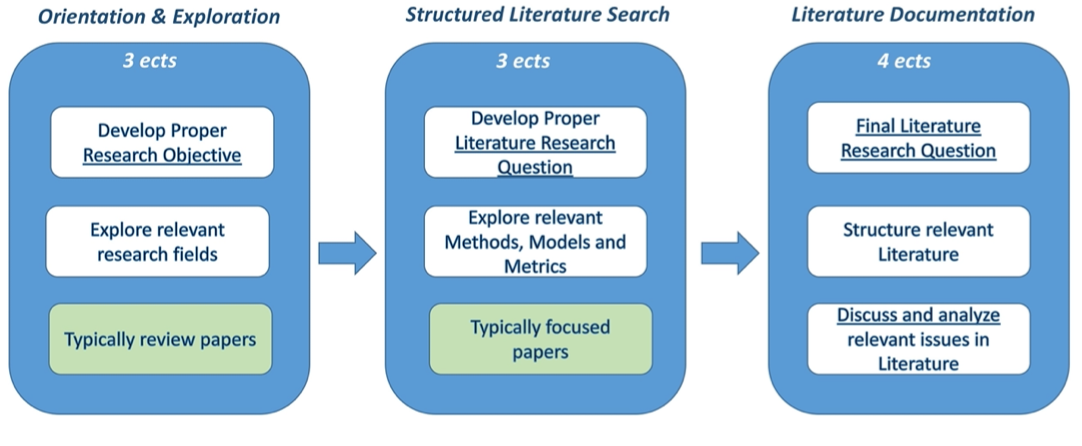
\includegraphics[width=0.8\textwidth]{figures/literatu_study_process.png}
	\caption{Overview of the literature study, reproduced from \cite{Master Thesis Guide, HRI section Cognitive Robotics}.}
	\label{fig:dexnet3_functionality}
\end{figure}

\section{Literature Review in the MSc Robotics program}
The Literature Review is called the Literature Research in the MSc Robotics Program, and it is 10EC
In detail, from the Study Guide \url{https://studiegids.tudelft.nl/}:

\begin{quote}
The aim of the literature study is to learn how to independently search for recent scientific publications (i.e., articles, theses, books). The literature study is carried out individually. The topic of the literature study is linked to the graduation project. The findings from the literature study are used to motivate the research plan of the thesis and are instrumental for achieving a high-quality final thesis.
\end{quote}

Learning Objectives:
After completing their literature research, students will be able to:
\begin{itemize}
    \item study a topic by critically selecting relevant scientific literature,
    \item identify and acquire lacking expertise
    \item identify the most interesting and relevant questions or problems in the field of the MSc thesis
    \item analyse and solve engineering problems in a systematic way
    \item present and report in good English
\end{itemize}

This part of your graduation process includes the following activities which are assessed:
\begin{itemize}
    \item Literature Research (written report; minimum grade: 6.0). The report is graded by the supervisor.
    \item Presentation (colloquium) (pass/fail). The presentation is combined with the introductory phase of the MSc project. The colloquium is graded by an ad-hoc committee of scientific employees of the department.
    \item Colloquium Attendance (pass/fail). All students must attend at least 10 colloquia.
\end{itemize}
	
\section{Literature Review at KAS Lab}


\chapter{Master Thesis}\label{c:msc_thesis}


In your MSc project you will complete your own scientific research project. In collaboration with your supervisors and the rest of the KAS Lab, you will define a research question and answer it using the proper scientific methods.

% Generally, a MSc project involves a human factors experiment, however every project is different and therefore there is no manual how-to-perform-a-master-thesis set in stone. Nonetheless, below we provide a general guide with some tips and tricks that usually apply.

\subsection{Step 1. Exploratory phase}

Even if you performed your literature study at the KAS Lab and had regular meetings with your supervisors, it is good to make an appointment to brainstorm about the topic of your master project. The \textbf{goal of this meeting is to brainstorm about the objective of the project}, and to find a direction that is interesting for both you and your supervisor. It is very well possible that during the first meeting you will not be able to make a decision on the topic yet. It probably takes some more deliberation, (re)reading of papers, and discussion before you can really settle on a topic.

\subsection{Step 2. Analysis phase – Research proposal}

\subsubsection{Research objective and question}
A good way to start your report is to write down your research objectives. This is usually done in a research proposal. In a research proposal you introduce a problem, motivate why it is important, and define your research objective.
Consider the research proposal as a living document, meaning it is best to update it as you go. It will start out as a draft and you can edit sections as you make progress. That is, during your thesis, you will be able to identify the problem you are investigating more specifically, which means you can make your introduction more focused, which in turn means you can delineate you research question, which determines your approach. A well updated research proposal can serve as a useful guide for your supervisory meetings. Moreover, when you will start writing your thesis, you will find that the proposal is a basis for your introduction and method section.

THE TIPS FROM HRI DO NOT APPLY DIRECTLY, BUT MAYBE WE COULD HAVE SOMETHING SIMILAR

OVERALL, THIS CHAPTER NEEDS TO ADAPT TO OUR RESEARCH 


\subsubsection{Hypotheses}
Every experiment starts with well-defined hypotheses. A hypothesis is an educated prediction of your experiment results. A good hypothesis is based on solid argumentation. Hypotheses can be based, for example, on previous literature or the results of a (small) Simulink modelling study.


\subsubsection{Methodology}
The scientific methods that you will use during the master project are mostly dependent on the objective. If your project is focused on design you will probably use a different approach than a thesis focused on analysis.
Initially, the approach will be a general description of the methods that you will use. For example, “To answer the sub-question 1, I will model the novel controller in Simulink in order to predict its behavior”. However, when your project progresses this section will become more specifically defined and will become more like the method section of a scientific paper.

\subsection{Step 3. Design and perform experiments}

% Like all the previous steps, designing an experiment is an iterative process. At the end of your analysis phase you will have a rough idea of the experiment you will be performing. Now is the time to hammer out the details:
% 1. Make a rough plan of the number of participants, which (in)dependent measures you will use, time the experiment will take etc.
% 2. Start to set-up the experiment. You will probably come across matters that will influence your experiment design. Meanwhile you specify the experiment in more detail.
% 3. Do pilot studies, which you will use to test the experiment design and gather some pre- liminary data.
% 4. Perform the experiment.



\section{Step 5. Writing report}
The general approach within the KAS Lab is to write it in the form of a paper, with additional background information in separate Appendices.

The paper is usually somewhere between 10 – 12 pages long. At first it might seem easy to fill these pages, but it is not about meeting the minimum amount of words. It is about conveying the most important message of your research, while providing the right amount of details. Con- sequently, condensing 6 months of work into 12 pages is actually pretty hard. Generally, a paper consists of the following sections:

ADAPT

\begin{itemize}
    \item Title
    \item Abstract
    \item Introduction
    \item Methods
    \item Results
    \item Discussion
    \item Conclusion
    \item References
    \item (Author biographies)
\end{itemize}

 TIP: 
Examples of MSc theses can be found in the TU Delft Repository. We have also included a couple of good examples in the starter pack (see 01 Literature).
This paper provides an excellent set of principles and tips for structuring and writing your paper. Highly recommended!
This other link provides useful tips and tricks for writing a paper and presenting figures and tables. Note that some tips are very specific for publishing in journals, these can be ignored.
Use a decent spelling and grammar check on your report (especially before handing it in). Grammarly is a good choice (the paid version has additional checks, but the free version works fine too).


Reporting Tips from \href{https://biaslab.github.io/research/starter-guide/}{https://biaslab.github.io/research/starter-guide/}

Start working on the final report in the first month of the project. In particular, if you follow Magnusson’s advice to write backward (start with the conclusions!), then you can turn report writing into a powerful research tool that reveals your next steps to pursue. I strongly encourage you to have a look at Simon Peyton Jones’ lectures on writing a paper (video and slides) and giving a talk (video and slides).

In general, if you work on an MSc thesis project or higher, I’d like you to make a (final) report update at least once a month. The final report should be in the form of a publishable IEEE journal paper. So, working on a project implies a monthly refinement of the paper until it’s ready for submission (or project time runs out). Use the process of incremental report refinement as a tool to discover what you need to work on next.


\section{Step 6. Final presentation and defence }
The graduation event consists of:

\begin{itemize}
    \item Public presentation (20min + 10min questions)
    \item Private defence, a.k.a exam instruction
    \item Graduation diploma and celebration
\end{itemize}

\subsection{Requisites and organization of MSc graduation}

Before your graduation, you need to make certain criteria and organise your graduation event. Note that the CoR secretary and your supervisors at KAS Lab will help you with organizing the event, but you are responsible for it, so do not wait for others (e.g. your supervisors) to make it happen.

Checklist and actions before your defence (just an orientation, the MSc official regulations rule):

\begin{itemize}
    \item Check the official requirements and process from the MSc Robotics regulations and follow those when in conflict with this list!
    \item Green-light: organize a meeting with your supervisors where you prove to them that you are ready to organize your defence and celebrate it in ~4 weeks
    \item Check that you have all credits required approved in OSIRIS (courses, internship, literature review \dots)
    \item Make sure your supervisor's contact committee members and find a suitable graduation date.
    \item Submit a copy to the committee members at least 2 weeks before the graduation date
    \item Invite your family, friends, classmates, and KAS Lab members (at least) to your defence!!
\end{itemize}





\subsection{Public MSc presentation}

In a 20-minute presentation, you present your main findings to your family, classmates, and committee. Such scientific presentation typically consists of the following parts - REVIEW text from HRI:

\begin{itemize}
    \item Title slide: The first slide contains the title, name, date and (optional) your committee members.
    
    \item Introduction: Why did you investigate the problem?
Start by motivating the problem you investigated by introducing it in a larger context. A good introduction starts broad and narrows it down until the research question you investigated.

    \item Method: How did you investigate the problem?
In the method, you explain the details the research approaches you used. The trick is to present the most important details of your work, while still keeping it understandable for your audience.
    \item Results/Discussion: What did you find?
Show the most important results here and highlight interesting findings. Again, balance is key in present your results with enough detail, so that your conclusions make sense, but avoid losing the key message in graphs and tables. Do not only present the results, but discuss what they mean in light of your research question.

    \item Conclusions: The conclusions summarize the findings of your study for the audience. What is important for the audience to remember?
    
    \item Future work: So now what?
Place your MSc project in a larger context. What does your work and your conclusions mean for the field and how should future research use it?

    \item Take home message: (optional) End your presentation with a nice take home message. The last part of the presentation is often what the audience will remember, so make it last.

\end{itemize}

To practice for your presentation, in addition to the MSc Robotics Literature Colloquia, we have the joint supervision KAS Lab bi-weekly meetings.
We require you to present multiple times during your graduation process in those meetings: in the "updates meetings", to briefly (5-7 min, ~3 slides) share your progress with your project, and longer (20min) to discuss in depth scientific questions and challenges that you encounter.
But make sure to reserve a spot to present your graduation project in such a meeting one or two weeks before your graduation defence.

\subsection{Private defence and evaluation}
The Private defence is an approximately 1h close-door scientific discussion of the MSc student with the graduation committee, who pose questions to the student about the graduation project, its scientific contributions, the methods used and the connection to knowledge the student is expected to have acquired during the entire education in the MSc Robotics, meaning not only the graduation project itself but also the courses.

\subsubsection{Evalution and Feedback}
After the private defence, the committee deliberates to agree on a grade for the graduation project. For this assessment and posterior feedback to the student, they use the Master Thesis Graduation Rubric for the Faculty of 3mE (\href{link to forms}{https://www.tudelft.nl/en/student/faculties/3me-student-portal/education/related/student-forms/msc-forms/})

\subsection{Graduation diploma and celebration}
Congrats!!
You get a well-deserved diploma and a celebration! Do not forget to arrange for the celebration yourself, or get someone who likes you very much to do it for you;-)

\chapter{Data Management}\ref{c:data_management}

%% Use letters for the chapter numbers of the appendices.
% \appendix

% \input{appendix-a}

\printbibliography

\end{document}

